%%
%%   Version 3.1 of 16 May 2019.
%%
\documentclass[aip,jcp,amsmath,amssymb,reprint,floatfix]{revtex4-1}

\usepackage{graphicx}% Include figure files
\usepackage{dcolumn}% Align table columns on decimal point
\usepackage{bm}% bold math

% hyphenation
\usepackage{hyphenat}

% tables
\usepackage{multirow}
\usepackage{booktabs}

% mathematics
\usepackage{amsmath}
\usepackage{amsfonts}
\usepackage{amssymb}
\usepackage{amsbsy}
\usepackage{mathrsfs}
\usepackage{upgreek}
\usepackage[cbgreek]{textgreek}

%---------------------------------------------------
% Approximations
\newcommand{\Approx}[2]{\ensuremath{\text{Ap}_{#2} \left[ {#1} \right] }}
% happy integral
\newcommand{\rint}[1]{\mbox{\Large $ \int\limits_{\mbox{\tiny  $#1$}}$}}
% SHORTCUTS
%\newcolumntype{,}{D{.}{,}{2}}
\newcommand{\citee}[1]{\ensuremath{\scriptsize^{\citenum{#1}}}}
\newcommand{\HRule}{\rule{\linewidth}{0.2mm}}
% Quantum notation
\newcommand{\Bra}[1]{\ensuremath{\bigl\langle {#1} \bigl\lvert}}
\newcommand{\Ket}[1]{\ensuremath{\bigr\rvert {#1} \bigr\rangle}}
\newcommand{\BraKet}[2]{\ensuremath{\bigl\langle {#1} \bigl\lvert {#2} \bigr\rangle}}
\newcommand{\tBraKet}[3]{\ensuremath{\bigl\langle {#1} \bigl\lvert {#2} \bigl\lvert {#3} \bigr\rangle}}
%
\newcommand{\bra}[1]{\ensuremath{\bigl( {#1} \bigl\lvert}}
\newcommand{\ket}[1]{\ensuremath{\bigr\rvert {#1} \bigr)}}
\newcommand{\braket}[2]{\ensuremath{\bigl( {#1} \bigl\lvert {#2} \bigr)}}
\newcommand{\tbraket}[3]{\ensuremath{\bigl( {#1} \bigl\lvert {#2} \bigl\lvert {#3} \bigr)}}
% Math
\newcommand{\pd}{\ensuremath{\partial}}
\newcommand{\DR}{\ensuremath{{\rm d} {\bf r}}}
%\newcommand{\BM}[1]{\ensuremath{\mbox{\boldmath${#1}$}}}
\newcommand{\BM}[1]{\bm{#1}}
% Chemistry (formulas)
\newcommand{\ch}[2]{\ensuremath{\mathrm{#1}_{#2}}}
% Math 
\newcommand{\VEC}[1]{\ensuremath{\mathrm{\mathbf{#1}}}}
% vector nabla
\newcommand{\Nabla}{\ensuremath{ \BM{\nabla}}}
% derivative
\newcommand{\FDer}[3]{\ensuremath{
\bigg(
\frac{\partial #1}{\partial #2}
\bigg)_{#3}}}
% diagonal second derivative
\newcommand{\SDer}[3]{\ensuremath{
\biggl(
\frac{\partial^2 #1}{\partial #2^2}
\biggr)_{#3}}}
% off-diagonal second derivative
\newcommand{\SSDer}[4]{\ensuremath{
\biggl(
\frac{\partial^2 #1}{\partial #2 \partial #3}
\biggr)_{#4}}}
% derivatives without bound
% derivative
\newcommand{\fderiv}[2]{\ensuremath{
\frac{\partial #1}{\partial #2}}}
% diagonal second derivative
\newcommand{\sderiv}[2]{\ensuremath{
\frac{\partial^2 #1}{\partial #2^2}
}}
% off-diagonal second derivative
\newcommand{\sderivd}[3]{\ensuremath{
\frac{\partial^2 #1}{\partial #2 \partial #3}
}}
% derivatives for tables
\newcommand{\fderivm}[2]{\ensuremath{
{\partial #1}/{\partial #2}}}
% diagonal second derivative
\newcommand{\sderivm}[2]{\ensuremath{
{\partial^2 #1}/{\partial #2^2}
}}
% off-diagonal second derivative
\newcommand{\sderivdm}[3]{\ensuremath{
{\partial^2 #1}/{\partial #2 \partial #3}
}}
% ERIs and OEIs
\newcommand{\OEIc}[3]{\ensuremath{\left(#1 \lvert #2 \rvert #3 \right)}}
\newcommand{\ERIc}[4]{\ensuremath{\left(#1 #2 \vert #3 #4 \right)}}

% Partial density and potential
\newcommand{\PartPot}[4]{\ensuremath{\frac{#1 #2}{\lvert #3-#4 \rvert }}}

% trace operator
\DeclareMathOperator{\Tr}{Tr}

%\draft % marks overfull lines with a black rule on the right

% Define location of graphics
\graphicspath{{./figures/}}

\begin{document}
\preprint{AIP/123-OEP}

\title{Supplementary Information\\Ab Initio Effective One-Electron Potential Operators:
Applications for Charge-Transfer Energy in Effective Fragment Potentials}

\author{Bartosz B{\l}asiak}
\email[]{blasiak.bartosz@gmail.com}
\homepage[]{https://www.polonez.pwr.edu.pl}

\author{Joanna D. Bednarska}
\author{Marta Cho{\l}uj} 
\author{Wojciech Bartkowiak}

\affiliation{Department of Physical and Quantum Chemistry, Faculty of Chemistry, 
Wroc{\l}aw University of Science and Technology, 
Wybrze{\.z}e Wyspia{\'n}skiego 27, Wroc{\l}aw 50-370, Poland}

\date{\today}

\pacs{}

\maketitle

\tableofcontents

\section{Asymptotic dependence of CT interactions for methanol-water complex}

%
\begin{figure}[h]
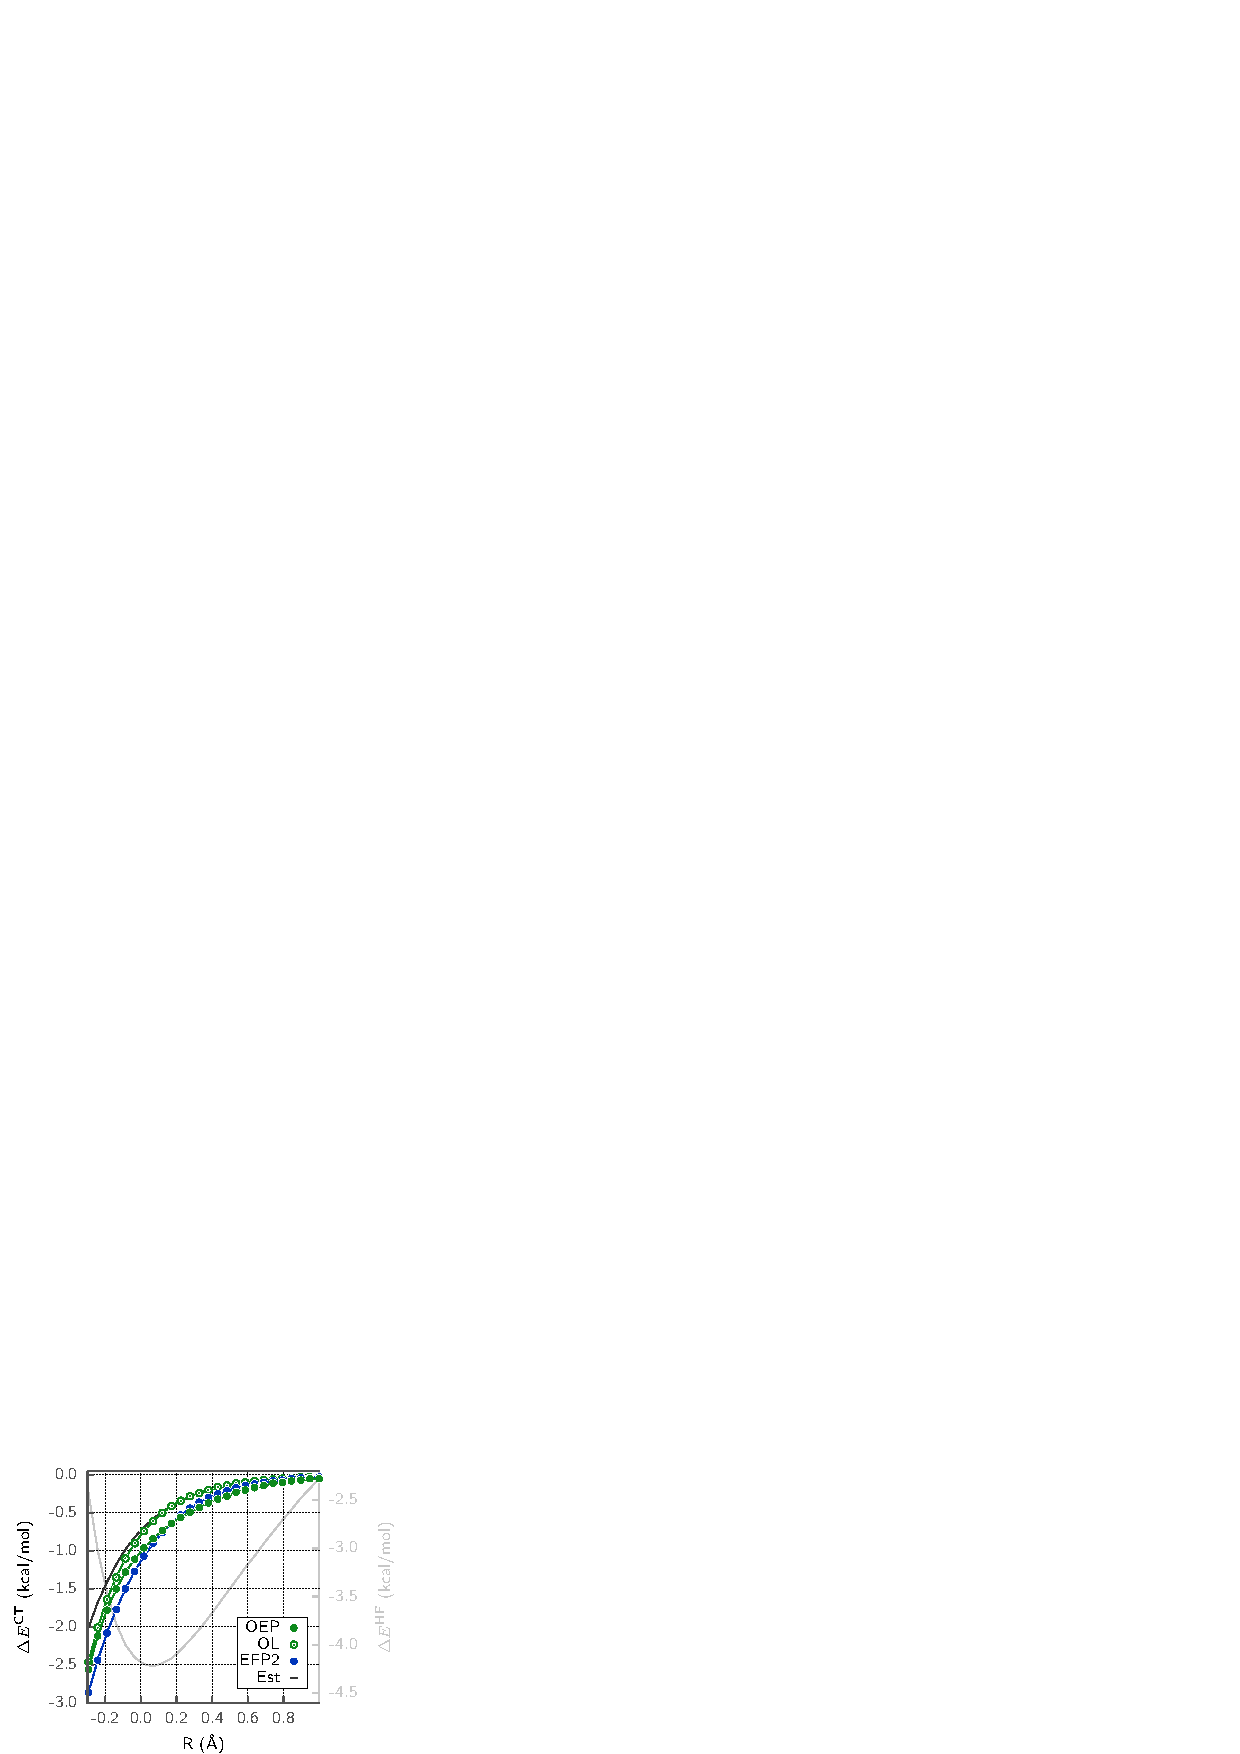
\includegraphics[width=0.5\textwidth]{fig-s1.pdf}
\caption{\label{f:fig-s1} {\bf Asymptotic dependence of the charge transfer energy
in the CT/HF0 formulation for water-methanol complex.} 
Water molecule has been translated by $R$ from the starting geometry
along the vector specified in the inset picture.
The counterpoise\hyp{}corrected total interaction energy
is also shown for comparison in light grey color in this figure.
All data were obtained at HF/6-311++G(2df,2pd) level of theory
with the single GDF scheme and aug-cc-pVTZ-jkfit auxiliary basis set.
} 
\end{figure}
%


\section{Statistical validation of OEP method}

% -----------------------
\bibliography{references}
% -----------------------

\end{document}
